\title{PS1 Solutions}

%TEMPLATE HEADER
%This is the homework solution template
\documentclass[11pt]{article}

%AMS-TeX packages
\usepackage{amssymb, amsmath, amsthm} 
\usepackage[margin=.75in]{geometry}
\usepackage{graphicx}
\usepackage{caption}
\usepackage{subcaption}
\usepackage{bm} % bold math

%Redefining sections as problems
\makeatletter
\newenvironment{problem}{\@startsection
       {section}
       {1}
       {-.2em}
       {-3.5ex plus -1ex minus -.2ex}
       {0.2ex plus .2ex}
       {\pagebreak[3]%forces pagebreak when space is small; use \eject for better results
       \Large\sc\noindent{Problem }}\\}
\makeatother

%Fancy-header package to modify header/page numbering 
\usepackage{fancyhdr}
\pagestyle{fancy}
\lhead{\textbf{Ge/ESE 118}} %name of the course
\chead{\textbf{}} %topic of the homework set
\rhead{\textbf{Solution 1}} %number of the homework set
\lfoot{}
\cfoot{}
\rfoot{\thepage}

%Include frequently used commands used for equations
%Fractions
\newcommand\fr[2]{\frac{#1}{#2}} %Regular fraction

%Braces, Brackets, Parentheses, etc.
\newcommand\brcs[1]{\{#1\}} %Braces
\newcommand\brckts[1]{\left[#1\right]} %Brackets
\newcommand\lr[1]{\left(#1\right)} %Parentheses
\newcommand\abs[1]{\Big\lvert#1\Big\rvert} %Absolute value
\newcommand\ltwo[1]{\lVert#1\rVert_2} %L2-norm
\newcommand\linf[1]{\lVert#1\rVert_\infty} %L2-norm

%Linear algebra
\newcommand\tr[1]{\text{tr}\left( \mathbf{#1}\right)} %Trace
\renewcommand\det[1]{\text{det}\left( \mathbf{#1}\right)} %Determinant

%Trigonometric & special functions
\newcommand\sinb[1]{\, \sin\left(#1\right)} %Sine with parentheses: sin(x)
\newcommand\cosb[1]{\, \cos\left(#1\right)} %Cosine with parentheses: cos(x)
\newcommand\tanb[1]{\, \tan\left(#1\right)} %Tangent with parentheses: tan(x)
\newcommand\cotb[1]{\, \cot\left(#1\right)} %Cotangent with parentheses: cot(x)
\newcommand\sinc[1]{\, \text{sinc}\left(#1\right)} %Sinc function: sinc = sin(x)/x

%Calculus
\renewcommand\d[1]{\, \text{d}#1} %Differential for integrals
\newcommand\der[2]{\frac{\text{d}#1}{\text{d}#2}} %Ordinary derivate first order
\newcommand\dder[2]{\frac{\text{d}^2#1}{\text{d}#2^2}} %Ordinary derivate second order
\newcommand\od[3]{\frac{\text{d}^{#3}#1}{\text{d}#2^{#3}}} %Ordinary derivate any order
\newcommand\pder[2]{\frac{\partial#1}{\partial#2}} %Partial derivate first order
\newcommand\pdder[2]{\frac{\partial^2#1}{\partial#2^2}} %Partial derivate second order
\newcommand\pd[3]{\frac{\partial^{#3}#1}{\partial#2^{#3}}} %Partial derivative any order

%Fourier transform
\newcommand\ft[1]{\hat{#1}} %Fourier coefficient

%Probability theory, Statistics
\newcommand\ex[1]{\mathbb{E}\left[#1\right]} %Expectation
\newcommand\pr[1]{\mathbb{P}\left(#1\right)} %Probability
\newcommand\Var[1]{\text{Var}\left(#1\right)} %Variance
\newcommand\Cov[1]{\text{Cov}\left(#1\right)} %Covariance
\newcommand\one{\mathbf{1}} %Unity

%Miscellaneous 
\renewcommand\mod{\text{mod}} %Modulo

%CONTENTS OF THE HW SET SOLUTION BEGIN HERE
\begin{document}

\subsection*{Problem 1 (graded by Toby) - 30 points}
\subsubsection*{(a) 5 points}

The parameter vector is (in order) $m = [A, B, \omega, \phi, C, k]^T$.

\subsubsection*{(b) 5 points}

The gradient is (Here, $s$ stands for $\sin$ and $c$ for $\cos$)
\begin{equation}
\tiny{        \nonumber \nabla T =
\begin{pmatrix} 
1\\ 
c(\omega t + \phi)    (1+Cs(kx))   y\\
-Bs(\omega t + \phi)    (1+C s(kx))   yt\\ 
-Bs(\omega t + \phi)    (1+C s(kx))   y\\
B c(\omega t + \phi)    s(kx)   y\\
BC c(\omega t + \phi)    c(kx))   yx
\end{pmatrix}}.
\end{equation}

\subsubsection*{(c) 5 points}

The Hessian is symmetric if the derivatives with respect to different variables are interchangeble. This is true if the second derivatives are continuous (Schwartz's theorem) which is true in our case. This simplifies our life. The Hessian given in rows is given below
\begin{equation}
\tiny{
        \nonumber H =
\begin{pmatrix} 
0 & 0 & 0 & 0 & 0 & 0\\
0 & 0 & -s(\omega t + \phi)   (1+C s(kx))  yt & -s(\omega t + \phi)   (1+C s(kx))  y) & c(\omega t + \phi)   s(kx)  y & c(\omega t + \phi)   c(kx))  yx\\
0 & -s(\omega t + \phi)   (1+C s(kx))  yt & -Bc(\omega t + \phi)   (1+C s(kx))  yt^2 & -Bc(\omega t + \phi)   (1+C s(kx))  yt & -Bs(\omega t + \phi)   s(kx)  yt & -BCs(\omega t + \phi)   c(kx)  yt & \\
0 & -s(\omega t + \phi)   (1+C s(kx))  y) & -Bc(\omega t + \phi)   (1+C s(kx))  yt & -Bc(\omega t + \phi)   (1+C s(kx))  y & -Bs(\omega t + \phi)   s(kx)  y & -BCs(\omega t + \phi)   c(kx)  y \\
0 & c(\omega t + \phi)   s(kx)  y & -Bs(\omega t + \phi)   s(kx)  yt & -Bs(\omega t + \phi)   s(kx)  y & 0 & B c(\omega t + \phi) c(kx) yx\\
0 & c(\omega t + \phi)   c(kx))  yx & -BCs(\omega t + \phi) c(kx)  yt & -BCs(\omega t + \phi)   c(kx)  y & B c(\omega t + \phi)  c(kx) yx & -BC c(\omega t + \phi) s(kx))   yx^2
\end{pmatrix}}.
\end{equation}

\subsubsection*{(d) 5 points}

No, for example because long term trends and either the diurnal or seasonal cycle are not included. Also, the model parameter won't be able to capture spatial veriability at scales other than $1/k$ well. One can modify the model by adding a term $D t$ that captures the global warming trend over the last 10 years or other periodic terms (with coefficients) that capture variability at different scales in space and time better. Eventually this would lead to a Fourier representation of the temperature field.

\subsubsection*{(e) 5 points}
If only a linear trend is included, then there are 7 parameters. Otherwise, the number of parameters can vary greatly depending on the complexity of the modification.

\subsubsection*{(f) 5 points}
No, because there are more data points then model parameters. The resulting system of equations would be overdetermined. In this case we need to use a misfit measure, such as the $\mathcal{L}_2$-norm to determine the ``best'' possible set of parameters.

\newpage

\subsection*{Problem 2 (graded by Dunzhu) - 20 points}
\subsubsection*{(a) (4 points)}
\begin{equation*}
det
\begin{pmatrix}
1 & 1 & 1 \\ 3 & 2 &4 \\ 0 & 0 &1
\end{pmatrix} = 
1 \times 
det
\begin{pmatrix}
2 &4 \\ 0 &1
\end{pmatrix}
-1 \times 
det
\begin{pmatrix}
3 &4 \\ 0 &1
\end{pmatrix}
+1 \times 
det
\begin{pmatrix}
3 &2 \\ 0 &0
\end{pmatrix} = -1
\end{equation*}

Nonzero  $det(A)$ means A is invertiable. 

\subsubsection*{(b) (8 points)}
\begin{equation*}
det ( A - \lambda I ) = det 
\begin{pmatrix}
1-\lambda & 1 & 1 \\ 3 & 2-\lambda &4 \\ 0 & 0 &1-\lambda
\end{pmatrix} = 
det
\begin{pmatrix}
1-\lambda & 1  \\ 3 & 2-\lambda
\end{pmatrix} \times (1-\lambda) = 0  
\end{equation*}

so
\begin{equation*}
(\lambda^2-3\lambda-1)(\lambda-1) = 0
\end{equation*}
which gives the three eigenvalues.

To get corresponding eigenvectors, for each $\lambda_i$ solve
\begin{eqnarray*}
\begin{pmatrix}
1-\lambda_i & 1 & 1 \\ 3 & 2-\lambda_i &4 \\ 0 & 0 &1-\lambda_i
\end{pmatrix}
\begin{pmatrix}
x \\ y \\ z
\end{pmatrix} = 
\begin{pmatrix}
0 \\ 0 \\ 0
\end{pmatrix} 
\end{eqnarray*}

for $\lambda_1 = 1$, we have
\begin{eqnarray*}
y+z = 0 \\ 3 x + y + 4z = 0 
\end{eqnarray*}
one non-zero solution is $ x=1, y=1, z=-1 $. 

for $\lambda_2$ and $\lambda_3$, we have
\begin{eqnarray*}
(1-\lambda)x + y+z = 0 \\ 3 x + (2-\lambda)y + 4z = 0 \\ (1-\lambda) z =0 
\end{eqnarray*}
So we must have $z=0$. Then choose $x=1$, we have $y=\lambda-1$. Thus the three eigenvectors are
\begin{eqnarray*}
\begin{pmatrix}
1  & 1  & 1 \\ 
1  & (1+\sqrt{13})/2 & (1-\sqrt{13})/2 \\ 
-1 & 0 & 0
\end{pmatrix}
\end{eqnarray*}
Normalized it we get
\begin{eqnarray*}
\begin{pmatrix}
0.57735 & 0.39832 & 0.60890 \\
0.57735 & 0.91725 & -0.79325 \\
-0.57735 & 0 & 0
\end{pmatrix}
\end{eqnarray*}

\subsubsection*{(c) (4 points)}
It's equal up to numerical error.

\subsubsection*{(d) (4 points)}
The two matriices are similar. 


\newpage

\subsection*{Problem 3 (graded by Toby) - 20 points}

\subsubsection*{(a) (5 points)}

It implies that $\v{v}^T\v{x}$ = 0.

\subsubsection*{(b) (5 points)}

If $\v{v}_1$ and $\v{v}_2$ are in $\v{V}$ then using (a), we have that $\v{v}_1^T\v{x} = \v{v}_2^T\v{x} = 0$. Because the dot product is linear, we have $\left(a_1\v{v}_1 + a_2 \v{v}_2 \right)^T \v{x} = a_1\v{v}_1^T\v{x} + a_2 \v{v}_2^T\v{x} = 0 + 0 = 0$. Thus, $a_1\v{v}_1 + a_2 \v{v}_2$ is orthogonal to $\v{x}$ and by definition $a_1\v{v}_1 + a_2 \v{v}_2 \in \v{V}$. $\v{V}$ is called the orthogonal complement of $\v{x}$.

\subsubsection*{(c) (5 points)}

We have $\v{v} \in \v{V}$ and $\v{A}^T=\v{A}$. Thus, $(\v{A}\v{v})^T\v{x} = \v{v}^T\v{A}^T\v{x} = \v{v}^T\v{A}\v{x} = \lambda \v{v}^T\v{x} = 0$. Hence, we have that $\v{A}\v{v} \in \v{V}$.

\subsubsection*{(d) (5 points)}
The fundamental theorem of algebra implies that every matrix has an eigenvector because the characteristic polynomial has at least one solution. Let's call this guaranteed eigenvector $\v{x}_1$. 

\textbf{If the full vector space is one-dimensional}, we are done. If it has more then one dimension, we can pick a vector that is orthogonal to $\v{x}_1$, because the linear equation that is the orthogonality condition has infinitely many solutions. Let's call this orthogonal vector $\v{x}_2$. 

\textbf{If the full vector space is two-dimensional}, and using (c), we have that $\v{A}\v{x}_2 \propto \v{x}_2$, because $\v{A}\v{x}_2 \in \v{V}$. Thus $\v{x}_2$ is an eigenvector and we have found an orthogonal basis of eigenvectors, namely $\{\v{x}_1, \v{x}_2 \}$. 

\textbf{If the full vector space is three-dimensional}, the orthogonality conditions implies that there are two linearly independent vectors $\v{v}_1$ and $\v{v}_2$ that are both orthogonal to $\v{x}_1$. Using (b) and (c), we have that $\v{v}_1$ and $\v{v}_2$ span a suspace that is invariant under $\v{A}$. This implies that it contains at least one eigenvector (to be taken as given) that is orthogonal to $\v{x}_1$. We can call this eigenvector $\v{x}_2$ and it is orthogonal to $\v{x}_1$. Because the vector space is three dimensional, there must be vector that is orthogonal to both, $\v{x}_1$ and $\v{x}_2$ (two orthogonality conditions with three unknowns implying all vectors that are orthogonal to $\v{x}_1$ and $\v{x}_2$ span a one dimensional vector space). Applying (c) using both $\v{x}_1$ and $\v{x}_2$ simulataneously, we have constructed a vector $\v{x}_3$ with $\v{A}\v{x}_3 \propto \v{x}_3$. Thus we have constructed an orthogonal basis of eigenvectors, namely $\{\v{x}_1, \v{x}_2 , \v{x}_3\}$.

Repeat for higher dimensions according to the same recipe (induction). Because we can construct $n$ (where $n$ is the dimension of the full vector space) orthogonal eigenvectors this way, we have found an orthogonal basis of the vector space. We can use this basis to diagonalize $\v{A}$, because it consists of eigenvectors that are linearly independent.

\subsection*{Problem 4 (graded by Stephen) - 20 points}
\subsubsection*{(a) 10 points}

\begin{verbatim}
%define the function f(x)
function[output]=f(x)
output = x^4 + 4*x^3 - 48*x^2 - 48*x + 208;
end

%define the function g(x)
function[output]=g(x)
output = 4*x^3 + 12*x^2 - 96*x - 48;
end

%define the NewtonsMethod function
function [solution] = NewtonsMethod(tolerance,initialguess)
%uses Newton's method to find the zeros of fxn f(x)
xnew = 0;
xold = initialguess;
change = tolerance+1;

while(abs(change)>tolerance)
    xnew = xold - (f(xold))/(g(xold))
    change = xnew-xold
    xold = xnew
end
solution = xnew;


\end{verbatim}

\subsubsection*{(b) 10 points}
\begin{verbatim}
%use functions defined above to solve for zeros of f(x) using starting guesses from x=-15 to x=15
xrange=linspace(-15,15);
solutions=zeros(100,1);
for(i=1:100)
    solutions(i) = NewtonsMethod(0.0001,xrange(i));
end

plot(xrange,solutions,'.')
\end{verbatim}

\begin{figure}[htbp]
	\centerline{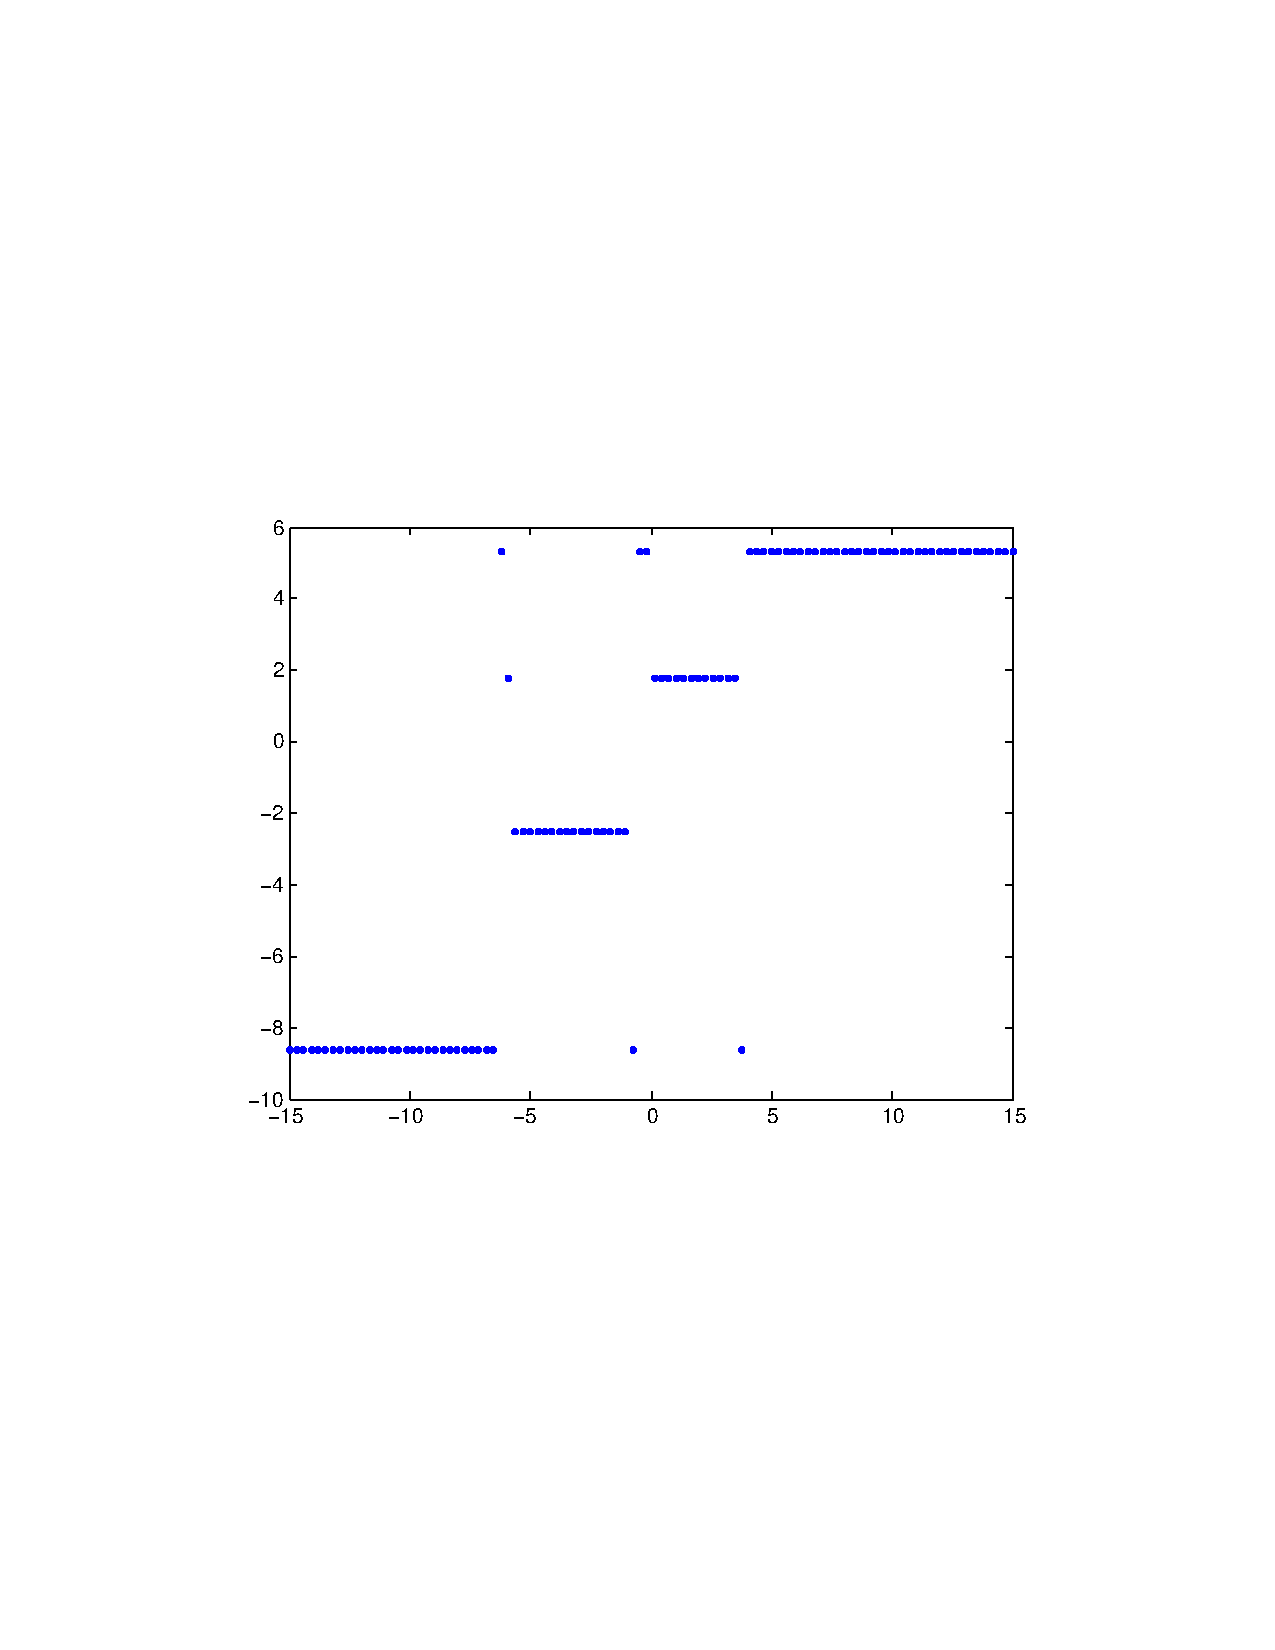
\includegraphics[width=1\textwidth]{newtonSolution.pdf}}
	\caption{\label{p1}%
	Plot of the Newton's method solutions (y-axis) vs. intial guesses (x-axis).}
\end{figure}

\begin{figure}[htbp]
	\centerline{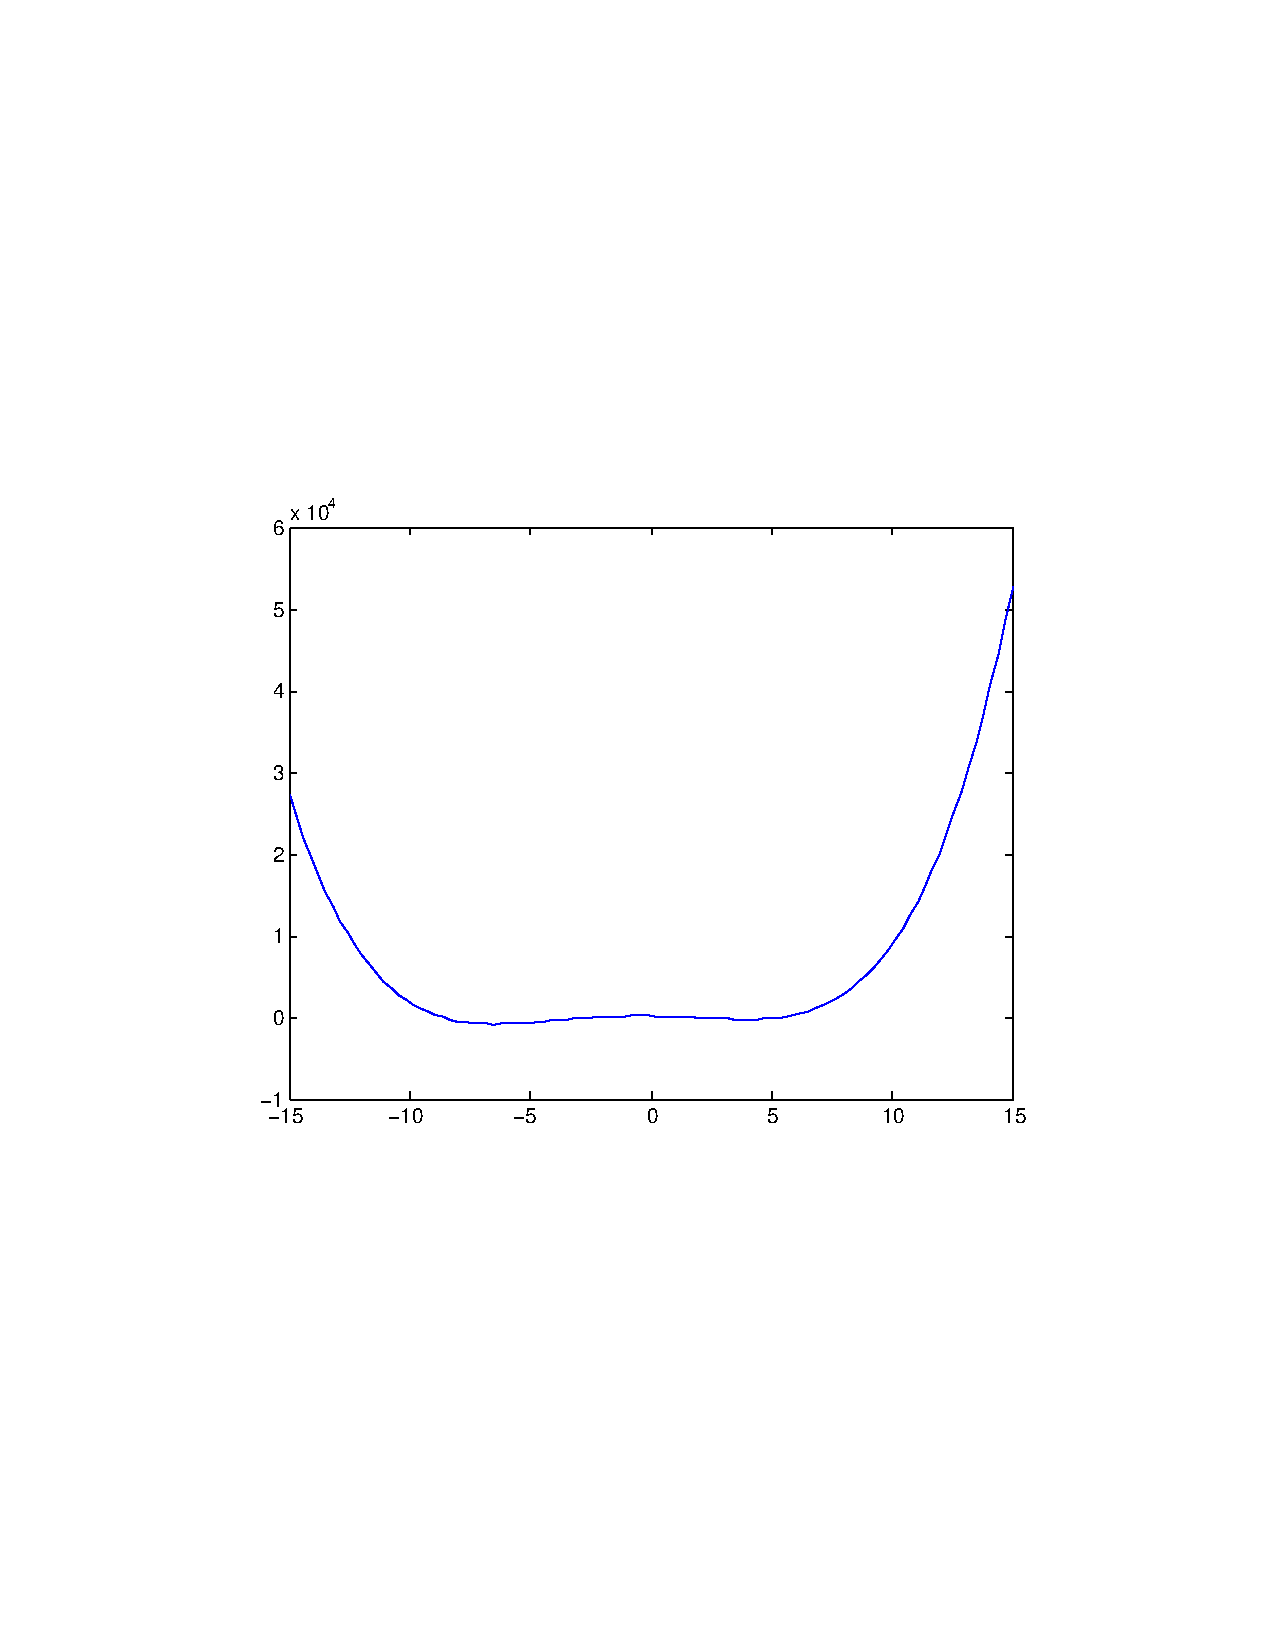
\includegraphics[width=1\textwidth]{fplot.pdf}}
	\caption{\label{p1}%
	Plot of the function f(x) over the range x=-15 to x=15.}
\end{figure}

\begin{figure}[htbp]
	\centerline{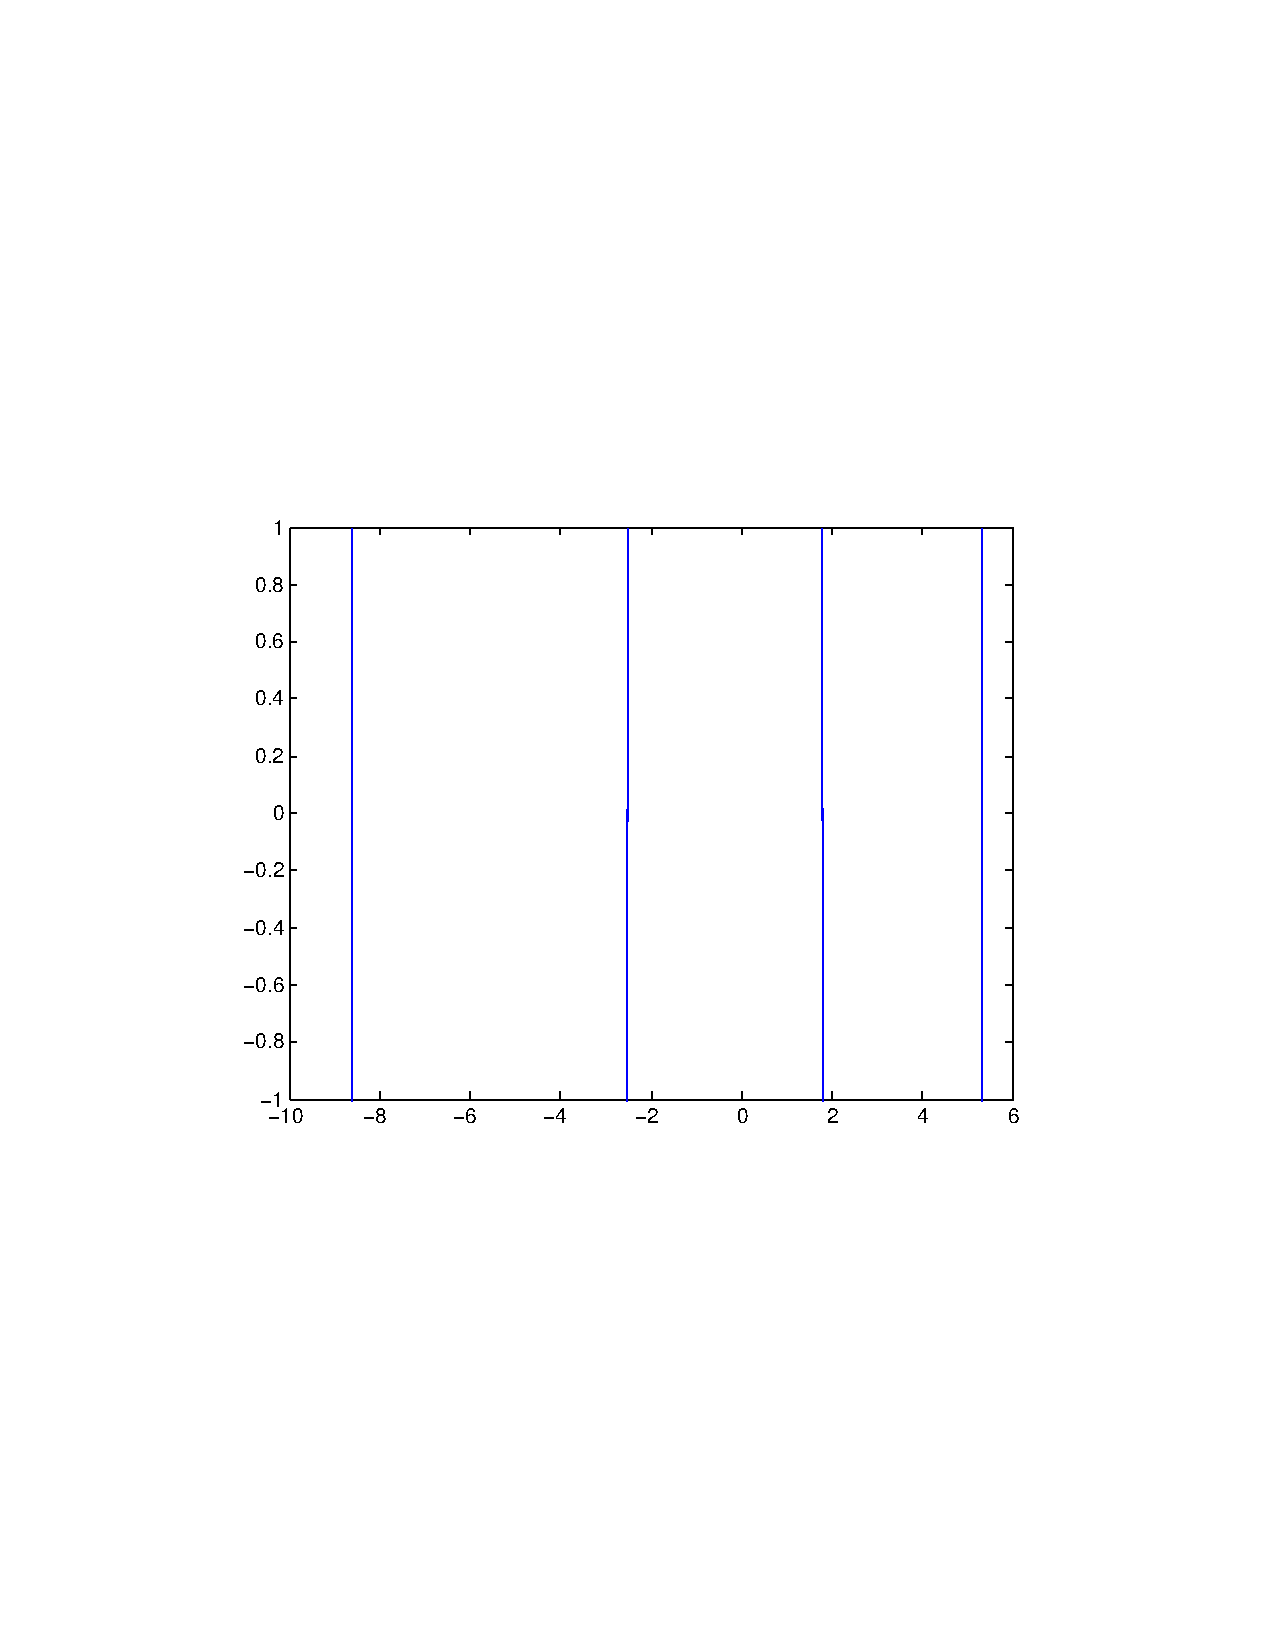
\includegraphics[width=1\textwidth]{zeros.pdf}}
	\caption{\label{p1}%
	Crop of the plot of f(x) over the range x=-15 to x=15 to show the zeros of the function at x=5.3267,1.7994,-2.5222,-8.6038}
\end{figure}

We see that our Newton's search converges a zero of the function every time.  Usually the search will converge to the nearest zero; however, for cases where we start near a minimum or maximum (ie. g(x)~0), the search may experience large intial changes and instead settle on one of the other zeros.  This can be seen for intial values near -6 and -1.  Thus, each time we run the method we will find out one specific zero, but we need to potentially cover a large range of initial guesses to find all of the zeros.


% EXAMPLE FOR INCLUDING MATLAB CODE
%\begin{verbatim}
%function [out, JN] = fun(theta, var0)
%%Check in input is of correct format
%if size(theta,1) > size(theta,2)
%    theta = theta';
%end
%
% Load the provided data file
%load('CDS150_Hmwk_Asst_5_data.mat');
%
% Calculate JN
%uk      = fliplr(vander(U));
%uk      = uk(:,1:length(theta));
%th      = repmat(theta, [N 1]);
%JN      = 1/N*sum((sum(th.*uk,2)-Y').^2); 
%
%% Calculate the function to be minimized
%out     = 0.5*N*log(JN) + 0.5/var0*sum(theta.^2);
%\end{verbatim}

% EXAMPLE FOR INCLUDING A FIGURE
%\begin{figure}[htbp]
%	\centerline{\includegraphics[width=1\textwidth]{gfx/p1d.eps}}
%	\caption{\label{p1}%
%	Data (blue dots) and most probable model mean value (red) for $\sigma_0^2 = 10$.}
%\end{figure}

% EXAMPLE FOR INCLUDING A TABLE
%\begin{table}[htbp]
%	\centering
%		\begin{tabular}{c|c|c|c|c|c|c|c|c}
%			d & $\hat{\theta}_0$ & $\hat{\theta}_1$ & $\hat{\theta}_2$ & $\hat{\theta}_3$ & $\hat{\theta}_4$ & $\hat{\sigma}^2$ & $\ln \text{EV}$ & $p(M_d|
%			D_N,\mathbb{M})$\\
%1 & 1.324 & 0.777 & - & - & - & 0.043 & 24.495 & 0.000 \\
%2 & 0.954 & 3.053 & -2.294 & - & - & 0.011 & 182.902 & 0.324 \\
%3 & 0.977 & 2.765 & -1.556 & -0.497 & - & 0.011 & 183.156 & 0.418 \\
%4 & 0.975 & 2.739 & -1.274 & -1.118 & 0.377 & 0.011 & 182.675 & 0.258
%		\end{tabular}
%	\caption{Posterior probabilities and parameters for $d=1, \dotsc, 4$ for $\sigma_0^2=1$}
%\end{table}	
			
\end{document}